\chapter{Backgrounds}
\label{ch:background}

Backgrounds to the detection of \nuebar{}
due to other physical processes
are classified by their coincidence statistics:
whether the physical process produces intrinsically-correlated events,
or whether the process produces only one event at a time
(or events with a long (\SI{>>1}{\milli\second}) coincidence time).

\section{Muon veto}
\label{sec:muonveto}

The Daya Bay experimental halls are located underground
to help shield the ADs from muons produced in the upper atmosphere by cosmic rays.
However, the overburdens of \SIlist{250;265;860}{\mwe}
for EH1, EH2, and EH3, respectively, do not block all of the muons.
When a cosmic-ray muon enters the LS or GdLS volume of the AD,
it creates a scintillation signal (and a smaller Cherenkov radiation signal)
that is proportional to the distance traveled
through the AD.
Given that in LS and GdLS, $\frac{dE}{dx} \approx \SI{2}{\mev\per\cm}$,
even a muon that only clips the corner of the AD cound easily deposit
more energy than the most energetic reactor \nuebar{} interaction,
providing a convenient discriminant for identifying muon interactions.
Additional muon tagging is provided by the water pool
surrounding the ADs in each EH.
These pools are divided by opaque Tyvek sheets into inner and outer regions
which are monitored by PMTs for Cherenkov radiation from muons.

In addition to themselves creating signals in the ADs,
muons also create other sources of background:
A muon which interacts inside the AD can occasionally produce
the rare unstable isotopes \li, \he, and \boron.
These isotopes can decay through processes that exactly mimic the IBD signature.
A muon can instead interact with the rock surrounding the EHs
and generate energetic ``fast'' neutrons,
which can penetrate the water shield and stainless steel vessel surrounding the ADs
(\cref{subsec:fastn}).
If the fast neutron collides with a nucleus inside the LS or GdLS,
it could produce a prompt signal, and then capture on H or Gd to produce
a delayed signal, again mimicking the IBD double coincidence signature.
Since these processes are highly correlated with muons,
an appropriate set of veto windows can greatly reduce their contamination of the data.

The muon veto window procedure consists of four independent criteria
for classifying muons.
Most muons cause significant PMT signals in the inner and outer water shields.
Any event that triggered $>12$ PMTs in the inner water shield
is an inner water shield muon,
and any event triggering $>15$ PMTs in the outer wanter shield
is classified as an outer water shield muon.
A veto of \SI{400}{\micro\second} is applied to the data following
both types of water shield muons.
This veto is long enough to allow most (all but $\sim e^{-2}$)
fast neutrons that make it into the ADs to be captured by H or Gd
before the end of the veto window.
Since the time between water shield muons at the near halls
was only around \SI{5}{\milli\second},
extending the veto window much longer would lead to a significant
loss of data efficiency.
Both of these criteria have essentially \SI{100}{\percent} efficiency
in detecting muons.

Since muons deposit much more energy in ADs than most other processes,
a simple energy cut is used to identify so-called AD muons.
Any AD signal with a reconstructed energy of \SI{>20}{\mev}
is considered to be an AD muon, and is followed by a veto window
of \SI{800}{\micro\second}.
Some muons deposit significantly more energy than
even the maximum expected for a minimum-ionizing particle in LS
traversing the entire AD, approximately
approximately $\SI{6}{\meter}\times\SI{2}{\mev\per\cm}=\SI{1200}{\mev}$.
These events are assumed to be caused by muons which create particle showers,
explaining the additional energy deposits.
However, these particle showers also produce a much higher rate of
\li, \he, and \boron.
Because \li{} in particular has a rather long lifetime of \SI{257.2}{\milli\second},
the veto window for showering muons is extended to \SI{1}{\second}
to allow all but $\sim e^{-4}$ of the \li{} to decay before the veto window ends.

The muon veto also interacts with the coincidence selection,
as was mentioned in \cref{sec:coincidence}.
If a candidate coincidence window includes a muon event,
then all of the events in the coincidence window are vetoed.
This avoids an unwanted correlation between muon rate
and coincidence distance-time (DT) efficiency,
as would happen if instead of vetoing the window,
the window were simply truncated and accepted.
Because of this implicit pre-muon veto window,
an isolated water shield muon actually vetoes \SI{1900}{\micro\second}
of DAQ live time (given $\tc=\SI{1500}{\micro\second}$),
an AD muon vetoes \SI{2300}{\micro\second},
and a showering muon vetoes \SI{1.0015}{\second}.

When performing the event selection, no events which are vetoed by muons
are considered.
In order to form rates, the muon-corrected live time must be computed.
This live time is simply the total amount of time that
does not lie within any muon veto windows (including pre-muon veto windows).
The fraction of DAQ live time that is not vetoed
is the muon veto efficiency $\varepsilon_\mu$, not to be confused
with the fraction of muons which are vetoed,
which is taken to be \SI{100}{\percent}.
The muon veto efficiency over time for the near and far halls
is shown in \cref{fig:veto_eff} for each $\sim\SI{24}{\hour}$ data run.

\begin{figure}
    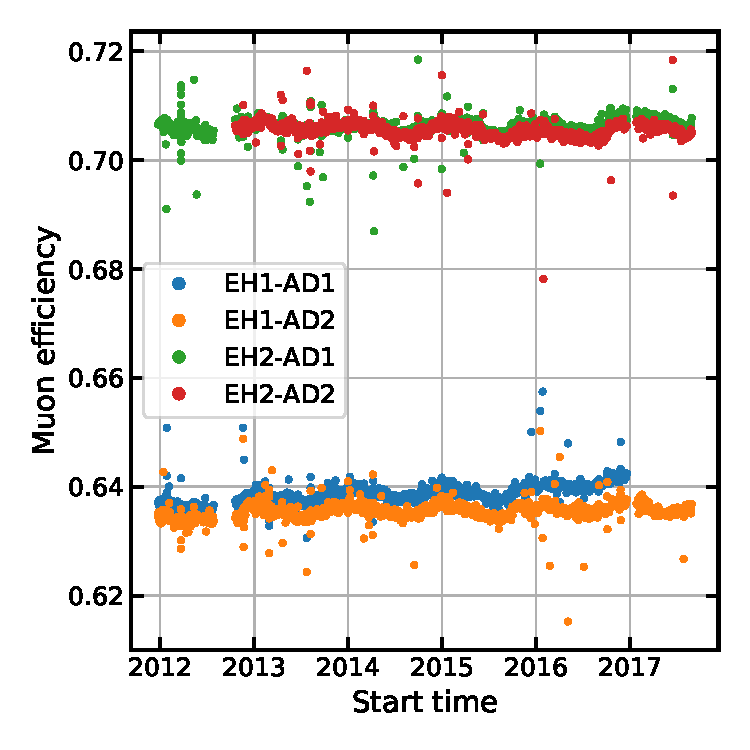
\includegraphics[width=0.48\textwidth]{plot_diagnostics/muon_eff_near_bydate}
    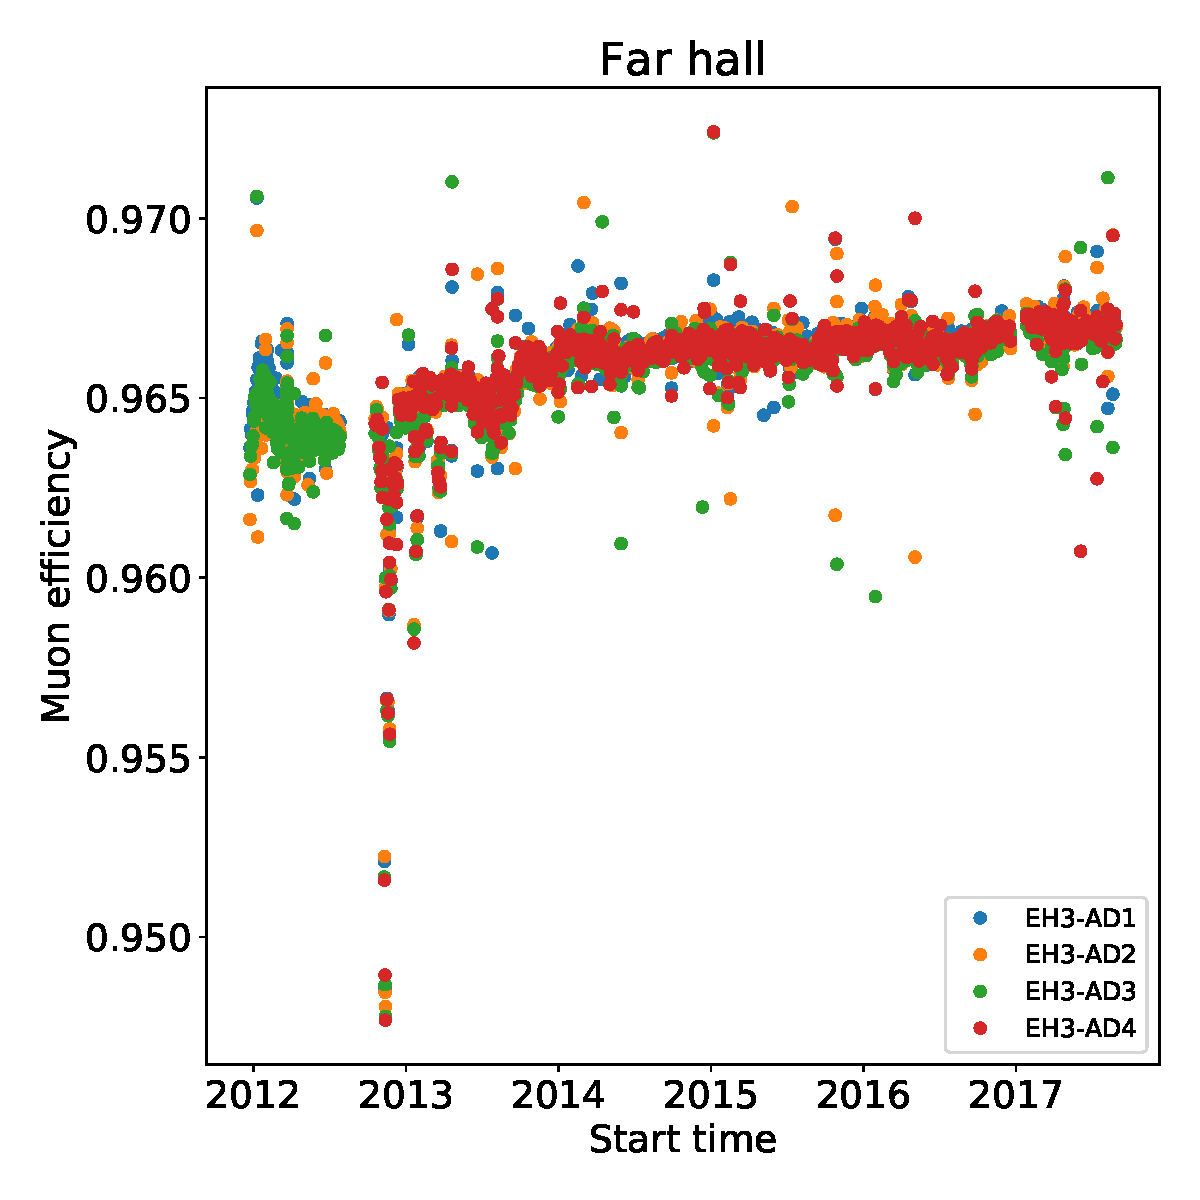
\includegraphics[width=0.48\textwidth]{plot_diagnostics/muon_eff_far_bydate}
    \caption{
        Muon veto efficiency $\varepsilon_\mu$ over time for
        the near halls (top) and far hall (bottom).
        Each data point represents one data run.
    }
    \label{fig:veto_eff}
\end{figure}

When determining the muon rate for the accidental background
analysis (\cref{subsec:acc}), overlapping windows are combined
into a single veto window.
Muon veto windows commonly overlap for a few reasons.
First, a single physical muon can create multiple muon events
that satisfy up to three of the four muon criteria,
if that muon creates signals in the inner and outer water shields,
and also enters an AD and deposits at least \SI{20}{\mev} worth of scintillation light.
Such a muon would then be an inner water shield, outer water shield, and AD
(or showering) muon.
Second, multiple muons can occur in quick succession,
such that the second muon occurs within the veto window of the first.
Lastly, muons can occur in not-quite-as-quick succession,
so that the pre-muon veto of the later muon overlaps with the
post-muon veto of the earlier one.
For example, consider two water shield muons occuring within \SI{1900}{\micro\second}.
Taking into account the implicit pre-muon veto
and given that $\tc=\SI{1500}{\micro\second}$,
any event occuring between those two muons will never be
a part of any coincidence group, not even a \fold{1} group.
Any event occuring in the first \SI{400}{\micro\second} would be vetoed outright
by the water shield muon veto.
And any event occuring in the latter \SI{1500}{\micro\second} would open a new
coincidence window, but that window would contain the second muon,
thus vetoing the original event.

\section{Uncorrelated background}

\subsection{PMT light emission / flashers}
\label{subsec:flashers}

\subsection{Accidental coincidences}
\label{subsec:acc}

Once muon events and flashers have been removed from the data stream,
the vast majority of remaining AD events are caused by uncorrelated
natural radioactive decays and are commonly known as ``singles,''
although as will be shown shortly, this name is misleading,
and a more appropriate name is ``uncorrelated events.''
These events occur at approximately \SI{19}{\hertz} in each AD and,
because they are uncorrelated, their groupings in time follow Poisson statistics.
In particular, there is a nonzero probability that
two of these uncorrelated ``single'' events will occur within
$\tc=\SI{1.5}{\milli\second}$ and thus form a \fold{2} coincidence.
In fact, for any given ``single'' event, the probability that
another ``single'' event will occur within \tc{} is

\begin{equation}
    \text{Poisson}(0\vert R_s\tc) = R_s\tc e^{-R_s\tc}.
\end{equation}
For the above value for $R_s=\SI{19}{\hertz}$, this probability is \SI{2.77}{\percent}.
Since \fold{2} coincidence groups like this are not formed from any
deliberate physical proccess but rather by an accidental coincidence,
they are known as the accidental background.
And these so-called ``singles'' events are not always alone;
they appear alongside other events rather frequently.
Crucially, though almost all \fold{1} coincidence groups
consist of a single uncorrelated event,
not all uncorrelated events form \fold{1} coincidences.
A back-of-the-envelope estimate of the rate of accidentals
gives an approximate rate of
$\SI{19}{\hertz}\times\SI{2.77}{\percent}=\SI{0.53}{\hertz}$
before applying the distance-time (DT) cut (\cref{sec:DT_cut}).

The full accidentals subtraction procedure begins with identifying
the rate of uncorrelated events in the AD, again better known
as the ``singles rate,'' for each individual data run.
The singles rate is measured by first measuring the rate of
\fold{1} coincidences in each run
(with the prompt energy bound of \SIrange{1.5}{12}{\mev}).
Given that rate, the true underlying rate of uncorrelated events can be
computed by numerically solving the following formula
(derived in \cref{ap:singlesformula}) for $R_s$:

\begin{align}
    \label{eq:rsingles}
    \begin{split}
        R_{\text{\fold{1}}}
          &= R_s e^{-R_s\tc}
          \left(
              e^{-(R_s + R_\mu)\tc} +
              \frac{R_s}{R_s+R_\mu} e^{-R_\mu\tc}
              \left(
                  1 - e^{-(R_s + R_\mu)\tc}
              \right)
          \right. \\
          &\ \ %
          \left. - \frac{R_s}{2R_s + R_\mu} e^{-R_\mu\tc}
              \left(
                  1 - e^{-(2R_s + R_\mu)\tc}
              \right) +
              \frac{R_\mu}{R_s + R_\mu}
              \left(
                  1 - e^{-(R_s + R_\mu)\tc}
              \right)
          \right)
    \end{split}
\end{align}
In this formula, \tc{} represents the actual duration of the coincidence window,
which technically begins \SI{1}{\micro\second} after the event,
meaning that a value of $\tc=\SI{1499}{\micro\second}$ should be used.
This formula is valid under the assumption that all \fold{1}
coincidences are formed from truly uncorrelated events.
Since the rate of correlated events like IBDs and other backgrounds
is \SI{<0.01}{\percent} the rate of correlated events,
this is an appropriate approximation to make.
The terms in brackets together represent the probability
that any given event does not fall in another event's coincidence window.
The leading term is simply the uncorrelated event rate $R_s$ times
the Poisson probability that no other uncorrelated event will occur
inside the given coincidence window.
The muon rate in this equation, $R_\mu$, is computed
by counting the number of muon veto windows in each run
after combining overlapping windows, and dividing by the muon-corrected
livetime.

\begin{figure}
    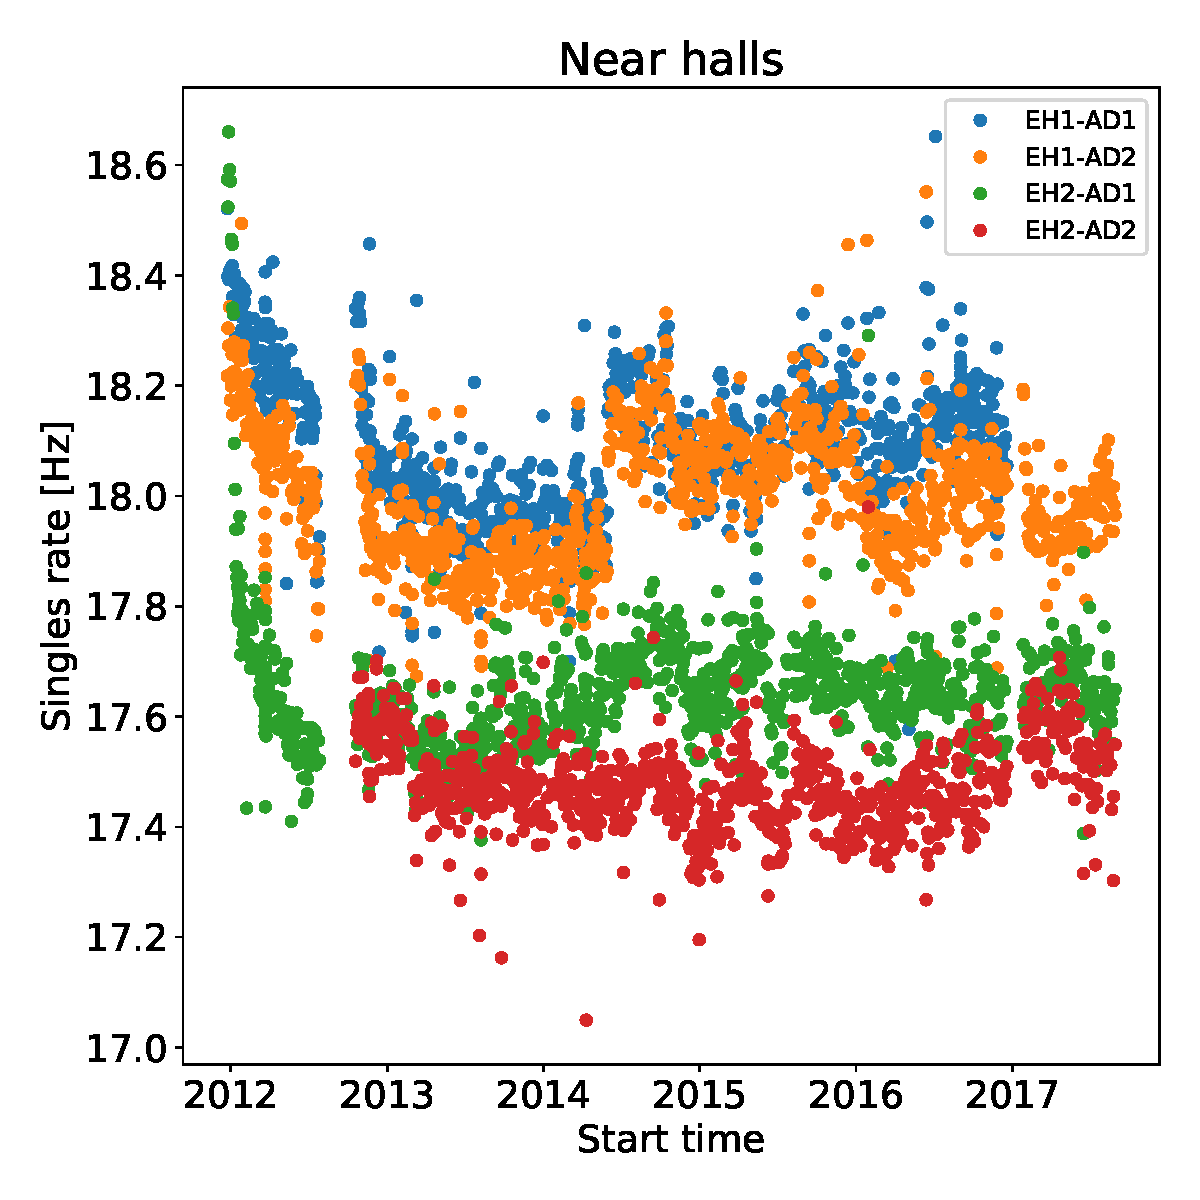
\includegraphics[width=0.48\textwidth]{plot_diagnostics/singles_near_bydate}
    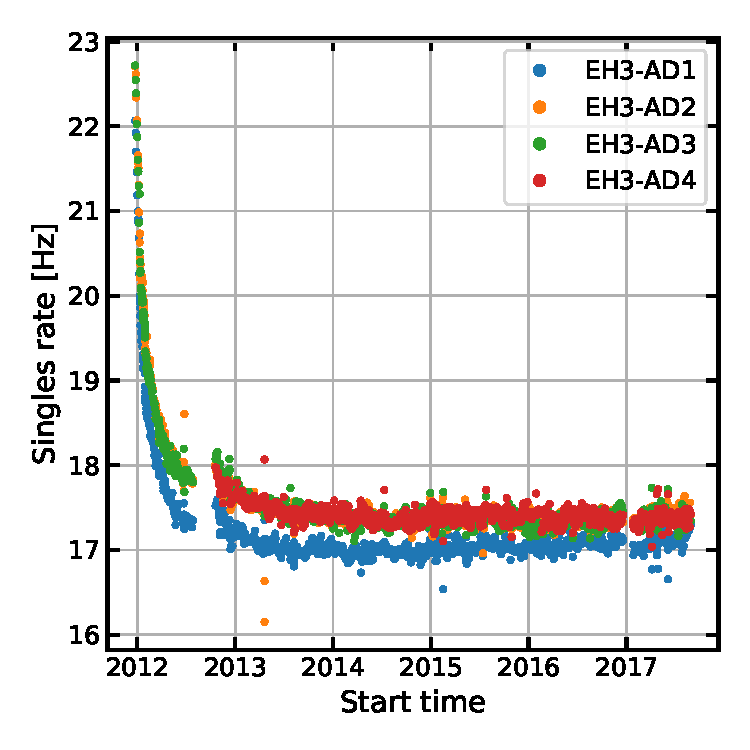
\includegraphics[width=0.48\textwidth]{plot_diagnostics/singles_far_bydate}
    \caption{
        Singles rate $R_s$ over time for
        the near halls (top) and far hall (bottom).
        Each data point represents one data run.
    }
    \label{fig:singles}
\end{figure}

The uncorrelated event rate $R_s$ for the near and far halls is shown in
\cref{fig:singles}.
$R_s$ was higher when the experiment began because long-lived
radioactive contaminants had not yet decayed away.
In particular, the far-hall ADs EH3-AD1, EH3-AD2, and EH3-AD3
were filled shortly before physics data taking began,
while the near-hall ADs EH1-AD1, EH1-AD2, and EH2-AD1
were filled and then studied for a few months
as part of detector commissioning, during which time
most of the radiocontaminants decayed.

Once $R_s$ is obtained, the rate of accidental coincidences $R_\fold{2}$
(before applying the rest of the event selection)
can be computed for each run
by simply adjusting the Poisson probability in \cref{eq:rsingles}
from the probability of $0$ other events within \tc{}
to the probability of $1$:

\begin{align}
    \label{eq:racc}
    \begin{split}
        R_{\text{\fold{2}}} &= R_s\tc R_{\text{\fold{1}}} \\
                   &= R_s \left(R_s\tc e^{-R_s\tc}\right)
          \left(
              e^{-(R_s + R_\mu)\tc} +
              \frac{R_s}{R_s+R_\mu} e^{-R_\mu\tc}
              \left(
                  1 - e^{-(R_s + R_\mu)\tc}
              \right)
          \right. \\
          &\ \ %
          \left. - \frac{R_s}{2R_s + R_\mu} e^{-R_\mu\tc}
              \left(
                  1 - e^{-(2R_s + R_\mu)\tc}
              \right) +
              \frac{R_\mu}{R_s + R_\mu}
              \left(
                  1 - e^{-(R_s + R_\mu)\tc}
              \right)
          \right)
    \end{split}
\end{align}

The rate $R_{\text{\fold{2}}}$ obtained from this formula
cannot simply be subtracted from the measured \fold{2} rate
to obtain $R_{\text{IBD}}$.
Most obviously, not all \fold{2} coincidence groups would be
mistaken for IBDs since some of them have delayed events that
do not satisfy the delayed energy cut.
In fact, \cref{subsec:delayed} makes clear that the delayed energy cut bounds
can only be determined after the accidental background spectrum
is subtracted from the measured spectrum of \fold{2} coincidences.
Thus it is necessary to measure the energy spectrum of
accidental coincidences.

Like the rate computation, the energy spectrum is determined for each run
by focusing on isolated events.
However, unlike the rate, a stricter isolation cut is used
to better ensure that only truly uncorrelated events are included in the sample.
This is acceptable because the characteristics of uncorrelated events
by definition do not change based on the presence or absence
of surrounding events.
A symmetrical isolation cut of $\tc=\SI{1.5}{\milli\second}$ is used
to ensure isolation before and after each candidate event.
The spectrum of these (now truly) single events is shown in \cref{fig:singlespectra},
obtained by summing the individual spectra from each data run.
%Prominent right at \SI{1.5}{\mev} is the tail of the
%reconstructed energy distribution for $\gamma$-rays associated with
%the decay of ${}^{40}\text{K}$ by electron capture.

\adgrid{Spectra of isolated single events in each AD.}{fig:singlespectra}{%
    ch_background/singles%
}

Uncorrelated events are not uniformly distributed
in position within the ADs.
Many of the radiocontaminants are on the surfaces of the
acrylic vessels that separate the mineral oil, LS, and GdLS regions.
To most accurately model the accidental background,
the singles sample is used to create a synthetic sample of accidental coincidences,
which is then used to actually perform the background subtraction
on the IBD candidates data set.
The synthetic accidental coincidence samples are formed for each run
by pairing up isolated events.
In particular, each isolated event is assigned an index in time order,
from $0$ to $N_{\text{isolated}}$.
Then each event $i$ from the first half is paired up with
the corresponding event $i + \nicefrac{N_{\text{isolated}}}{2}$.
The coincidence distance is taken to be the actual distance
between the reconstructed positions of the two events.
Each event pair generates two synthetic accidental events:
one with the event from the first half of the run as the prompt event,
and one with that event as the delayed event.
For each ordering and for each event pair, a coincidence time is chosen
uniformly at random to match the coincidence time distribution
expected from true accidental coincidences on the short timescale
of $\tc=\SI{1.5}{\milli\second}$.
From this synthetic accidental coincidence sample, $\varepsilon_{\text{DT,\,acc}}$,
the fraction of accidental \fold{2} coincidences which pass the distance-time (DT) cut,
can be computed.
And a prompt-delayed energy spectrum can be computed that only includes
synthetic accidental events which pass the DT cut. %TODO plots

Finally, an accidentals spectrum can be computed and subtracted
from the prompt-delayed spectrum measured from real data.
For each run, the expected number of accidental events that pass the DT cut is

\begin{equation*}
    N_{\text{acc}} = R_{\text{\fold{2}}} \times t_{\text{muon-corrected}}
        \times \varepsilon_{\text{DT,\,acc}}
\end{equation*}
The synthetic accidentals prompt-delayed spectrum, represented as a histogram,
is simply normalized so that the total number of entries is $N_{\text{acc}}$.
Then the histogram can be subtracted bin-by-bin from the corresponding histogram
representing the actual IBD candidates data sample.
The subtracted histograms are shown in Figure X. %TODO plots
These distributions, projected onto the delayed energy axis,
are used in \cref{subsec:delayed} to determine the delayed energy cut bounds.

The scale factor for the accidentals spectrum histogram,
$\nicefrac{N_{\text{acc}}}{N_{\text{acc,\,synthetic}}}$,
can be used to create histograms for other accidentals-subtracted quantities,
such as coincidence distance, DT, and 2D histograms of
those quantities' distributions with respect to prompt and delayed energy.
The accidentals-subtracted histogram of DT versus delayed energy
is used to compute the efficiency of the DT cut for IBDs in \cref{sec:DT_cut}.

\section{Correlated background}

\subsection{Muon-correlated backgrounds}
\label{subsec:li9}

\subsection{Fast neutrons}
\label{subsec:fastn}

\subsection{Am-C calibration source}
